% !TEX program = lualatex
\documentclass[12pt]{report}

% Font and layout
\usepackage{fontspec}
\IfFontExistsTF{Times New Roman}{\setmainfont{Times New Roman}}{\setmainfont{TeX Gyre Termes}}
\usepackage[a4paper,margin=1in]{geometry}
\usepackage{setspace}
\onehalfspacing
\usepackage{titlesec}
\titleformat{\section}{\bfseries\fontsize{14pt}{16pt}\selectfont}{\thesection.}{0.5em}{}
\titleformat{\subsection}{\bfseries\fontsize{13pt}{15pt}\selectfont}{\thesubsection}{0.5em}{}
\usepackage{hyperref}
\usepackage{xurl}
\hypersetup{colorlinks=true,linkcolor=black,urlcolor=blue,breaklinks=true}
\usepackage{graphicx}
\usepackage{array}
\usepackage{enumitem}
\setlist{noitemsep,topsep=2pt}
\usepackage{microtype}
\usepackage{booktabs}
\usepackage{tabularx}
\usepackage{float}
\usepackage{placeins}
\usepackage{newunicodechar}
\newunicodechar{‑}{-}
\setlength{\tabcolsep}{3pt}
% Ragged-right wrapped column type for tabularx
\newcolumntype{Y}{>{\raggedright\arraybackslash}X}
\usepackage{tikz}
\usetikzlibrary{shapes.geometric, arrows.meta, positioning, fit, backgrounds}
\usepackage{eso-pic}

% Convenience macros
\newcommand{\course}{BCSE401L -- Internet of Things}
\newcommand{\projecttitle}{An IoT-Based Indoor Air Quality Management System}
\newcommand{\institute}{Vellore Institute of Technology Vellore -- 632014, INDIA}
\newcommand{\dept}{Department of Computer Science \& Engineering}
\newcommand{\authors}{ARNAV SINHA -- 22BCE0830\\AKSHAT SINHA -- 22BCE2218}
\newcommand{\guides}{USHUS\\ELIZEBETH\\ZACHARIAH}
\newcommand{\reportdate}{30, October 2025}

\begin{document}

% Cover Page
\begin{titlepage}
% Add decorative border
\AddToShipoutPictureBG*{%
  \AtPageLowerLeft{%
    \begin{tikzpicture}[remember picture,overlay]
      % Outer border
      \draw[line width=2pt] 
        ([xshift=0.75cm,yshift=0.75cm]current page.south west) rectangle 
        ([xshift=-0.75cm,yshift=-0.75cm]current page.north east);
      % Inner border
      \draw[line width=0.5pt] 
        ([xshift=0.95cm,yshift=0.95cm]current page.south west) rectangle 
        ([xshift=-0.95cm,yshift=-0.95cm]current page.north east);
    \end{tikzpicture}
  }%
}
\centering
\vspace*{1cm}
{\large A\\[6pt] Final Project Report\\[6pt] Submitted}\\[12pt]
{\bfseries\Large in Fulfillment of the Requirements}\\[10pt]
{\itshape for the course}\\[4pt]
{\Large \course}\\[8pt]
{\itshape on the project entitled}\\[4pt]
{\bfseries\LARGE \projecttitle}\\[12pt]
{Submitted by}\\[6pt]
{\large \authors}\\[12pt]
{Under the guidance of}\\[6pt]
{\large \guides}\\[12pt]
\vfill
\IfFileExists{vit_logo.png}{\includegraphics[width=3cm]{vit_logo.png}\\[6pt]}{}
{\dept}\\[4pt]
{\institute}\\[6pt]
{\reportdate}
\end{titlepage}

\pagenumbering{roman}
\tableofcontents
\cleardoublepage
\pagenumbering{arabic}

% 0. Abstract
\section*{Abstract}
\addcontentsline{toc}{section}{0. Abstract}
This project presents a software-based indoor air quality (IAQ) monitoring system built using Internet of Things (IoT) technologies. The system tracks key air quality parameters including temperature, humidity, carbon dioxide (CO\textsubscript{2}), and particulate matter (PM2.5) in real time. We developed a complete solution with a FastAPI backend for data processing, SQLite database for storage, and a Streamlit web interface for visualization. The system implements India's Central Pollution Control Board (CPCB) National Air Quality Index standards for PM2.5 categorization and includes exposure time tracking across different pollution zones. Unlike hardware-dependent systems, our software-only approach uses simulated data generation with site-specific environmental profiles, making it accessible for testing and demonstration without physical sensors. The system successfully provides real-time alerts, historical trend analysis, and multi-site monitoring capabilities, addressing common challenges in IAQ management for homes, offices, and healthcare facilities.

% 1. Introduction
\section{Introduction}
We built a software-based indoor air quality (IAQ) monitoring system using Internet of Things (IoT) technologies. The system tracks temperature, humidity, CO\textsubscript{2}, and PM2.5 in real time and shows them through a clean web interface. This report documents the finished system, the design choices we made, and the results we observed while running it.

Indoor air quality has become increasingly important as people spend more than 90\% of their time indoors. Poor air quality can lead to health problems like respiratory issues, headaches, and reduced productivity. Traditional IAQ monitoring systems often require expensive hardware sensors and complex installation procedures, making them inaccessible for many users. Our project addresses this gap by creating a software-first solution that demonstrates how an IAQ system works without requiring physical sensors.

The system we developed consists of three main components working together. First, a data generation module creates realistic air quality readings that simulate different indoor environments like laboratories, classrooms, and canteens. Second, a backend API built with FastAPI processes this data, calculates air quality indices according to CPCB standards, and stores everything in a database. Third, a user-friendly web dashboard built with Streamlit displays the information through interactive charts, real-time metrics, and color-coded alerts. This architecture makes it easy to understand how data flows through an IAQ system and how different components interact with each other.

% 2. Motivation
\section{Motivation}
Clean indoor air is essential for health at home, work, hospitals, and elderly care. Since pollutants are invisible, we made IAQ visible and actionable through a simple dashboard and alerts. We aimed for a software-only build so the solution is easy to run and test without hardware.

We chose this topic because air pollution is not just an outdoor problem. Indoor spaces can trap pollutants from cooking, cleaning products, building materials, and even from people breathing. Carbon dioxide builds up in crowded rooms, particulate matter comes from dust and smoke, and humidity levels affect both comfort and mold growth. These invisible threats need to be monitored continuously, but most people cannot afford expensive sensor networks or do not have the technical knowledge to set them up.

Our motivation also came from seeing how IoT technology has made environmental monitoring more accessible. With affordable microcontrollers and wireless communication becoming common, the barrier to entry has lowered significantly. However, for students and researchers who want to learn about IAQ systems or test new algorithms, even these low-cost hardware solutions can be a hurdle. By creating a software-only system, we remove this barrier entirely. Anyone with a computer can run our system, experiment with different scenarios, and understand how IAQ monitoring works before investing in physical hardware. This educational aspect was particularly important to us as students learning about IoT systems ourselves.

% 3. Scope of the Project
\section{Scope of the Project}
\begin{itemize}
  \item We built a software-only IAQ system that collects, processes, and visualizes indoor air quality data.
  \item We let users access the data through a web portal with live charts and simple metrics.
  \item We included real-time alerts when air quality drops below safe levels.
  \item We store and display historical trends for better air quality management.
\end{itemize}
This helps building managers, healthcare workers, and residents.

The scope of our project covers several key areas. First, we focused on four critical air quality parameters: PM2.5 (fine particulate matter that can enter lungs), CO\textsubscript{2} (carbon dioxide indicating ventilation quality), temperature, and relative humidity. These parameters were chosen because they are the most commonly monitored in IAQ systems and have direct impacts on human health and comfort. We deliberately kept the parameter set manageable to ensure our system remains simple and easy to understand.

Second, we implemented multi-site monitoring capability, allowing the system to track air quality in different locations simultaneously. Each site (Lab, Classroom, Canteen) has its own environmental profile that generates realistic data patterns. For example, a canteen shows higher PM2.5 levels due to cooking activities, while a laboratory maintains cleaner air with better ventilation. This multi-site feature demonstrates how a real-world IAQ system would need to handle multiple sensors across different rooms or buildings.

Third, we integrated the CPCB National Air Quality Index specifically for PM2.5 monitoring. This means our system does not just show raw numbers but translates them into meaningful categories like Good, Satisfactory, Moderately Polluted, Poor, Very Poor, and Severe. Each category has a specific color code and health advisory, making it easy for non-technical users to understand the air quality status at a glance. We also track exposure time, showing how many minutes or hours were spent in each pollution category over the past day or week. This cumulative exposure data is more meaningful for health assessment than just looking at current readings.

What we deliberately excluded from scope: We did not implement actual hardware sensors, real-time hardware communication protocols like ZigBee or LoRa, battery power management, or physical installation considerations. We also did not include advanced features like machine learning predictions, automated HVAC control, or mobile app development. These exclusions were intentional to keep the project focused on demonstrating core IAQ monitoring concepts through software.

% 4. Literature Review
\section{Literature Review}
People spend more than 90\% of their time indoors, so IAQ matters for health, comfort, and productivity. Early IoT systems for Ambient Assisted Living (AAL) showed how low-cost sensors and gateways can deliver real-time data to the web and phones. Over time, research moved from basic monitoring to prediction and even automatic control. Below we summarize the core lines of work we studied and used to guide our build.

\subsection{Foundational AAL systems}
Marques and Pitarma~\cite{marques2016} introduced a pioneering IAQ monitoring system specifically designed for Ambient Assisted Living environments. The system architecture employed Arduino Mega microcontrollers as sensor nodes, each equipped with an SHT10 sensor for temperature and relative humidity measurement, an MQ7 electrochemical sensor for carbon monoxide detection, a T6615 NDIR (Non-Dispersive Infrared) sensor for CO\textsubscript{2} monitoring with a measurement range of 0--5000 ppm, and an LDR (Light Dependent Resistor) for luminosity assessment. The sensor nodes communicated via XBee modules implementing the IEEE 802.15.4 ZigBee protocol, achieving a wireless range of approximately 27 meters in indoor environments. The IAQ Gateway, built on a Wemos D1 Mini with ESP-8266EX chipset, aggregated data from multiple nodes and transmitted it via Wi-Fi (IEEE 802.11 b/g/n) to a MySQL relational database. The system provided dual interfaces: a web portal (IAQ Web) and an Android mobile application (IAQMobile) for real-time monitoring and historical data visualization.

The modular architecture demonstrated scalability for multi-room deployments, with each sensor node operating autonomously and the gateway supporting concurrent connections from multiple nodes. However, the authors identified critical limitations: the MQ7 sensor required manual field calibration with known CO concentrations, the LDR exhibited poor accuracy under varying lighting conditions, and the T6615 and MQ7 sensors consumed significant power (approximately 150 mW and 900 mW respectively), limiting battery-operated deployment scenarios. The centralized gateway architecture also introduced a single point of failure, where gateway malfunction would compromise the entire monitoring network. Despite these constraints, the system successfully demonstrated that low-cost, open-source IoT components could deliver functional IAQ monitoring for AAL applications, establishing a foundation for subsequent research.

\subsection{Predictive analytics during the COVID-19 period}
Mumtaz et al.~\cite{mumtaz2021} advanced the field by integrating machine learning algorithms for predictive IAQ analytics, motivated by the COVID-19 pandemic's emphasis on indoor air quality for respiratory health. The system expanded the sensor array to include MQ135 (NH\textsubscript{3}, NO\textsubscript{x}, benzene, smoke), MQ7 (CO), MQ2 (CH\textsubscript{4}, LPG), MQ136 (H\textsubscript{2}S), and a Plantower PMS5003 laser scattering sensor for PM2.5 measurement with a resolution of 1 µg/m\textsubscript{3} and range of 0--500 µg/m\textsubscript{3}. The IoT node utilized an ATmega328P microcontroller (16 MHz, 32 KB flash memory) paired with a NodeMCU ESP8266 Wi-Fi module for wireless data transmission at 2.4 GHz frequency.

The key innovation was the implementation of supervised learning models for IAQ classification and forecasting. A feedforward Neural Network with three hidden layers (64, 32, 16 neurons) using ReLU activation functions achieved 99.1\% classification accuracy across five IAQ categories (Excellent, Good, Moderate, Poor, Hazardous) on a dataset of 10,000 labeled samples. More significantly, a Long Short-Term Memory (LSTM) recurrent neural network with 50 memory cells and a lookback window of 24 time steps predicted future pollutant concentrations with 99.37\% accuracy (R\textsuperscript{2} score) and RMSE (Root Mean Square Error) values of 2.3 ppm for CO\textsubscript{2}, 0.8 µg/m\textsubscript{3} for PM2.5, and 0.4°C for temperature over a 30-minute prediction horizon. The LSTM architecture's ability to capture temporal dependencies in time-series sensor data enabled proactive interventions, allowing building managers to adjust ventilation rates before pollutant levels exceeded WHO (World Health Organization) or EPA (Environmental Protection Agency) thresholds.

The system transmitted data packets (approximately 256 bytes per reading) via MQTT protocol to a cloud server, with a configurable sampling interval of 1--10 minutes. Real-time alerts were triggered when pollutant concentrations exceeded predefined thresholds: CO > 9 ppm (8-hour average), CO\textsubscript{2} > 1000 ppm, PM2.5 > 35 µg/m\textsubscript{3} (24-hour average). However, the authors acknowledged challenges in widespread deployment requiring dense sensor networks, and noted that long-term monitoring (>6 months) faced sensor drift issues, with MQ-series sensors exhibiting baseline resistance changes of 10--20\% over time, necessitating periodic recalibration.

\subsection{Specialized particulate monitoring}
Marques et al.~\cite{marques2018} developed iDust, a specialized system focusing exclusively on particulate matter monitoring using the Plantower PMS5003 optical particle counter. This sensor employs laser scattering technology to differentiate particle sizes: PM1.0 (particles ≤1.0 µm diameter), PM2.5 (≤2.5 µm), and PM10 (≤10 µm), with concentration measurements in µg/m\textsubscript{3}. The PMS5003 features built-in temperature compensation and a measurement range of 0--500 µg/m\textsubscript{3} with ±10 µg/m\textsubscript{3} accuracy at concentrations below 100 µg/m\textsubscript{3}.

The system utilized a WEMOS D1 mini (ESP8266 at 80 MHz, 4 MB flash) as the processing and communication unit, with dimensions of 5.5 cm × 4.5 cm × 4.5 cm, making it suitable for discreet installation. The ESP8266's integrated Wi-Fi capability (802.11 b/g/n, 2.4 GHz) enabled direct connection to wireless networks without requiring a separate gateway. A notable user-experience feature was the Wi-Fi provisioning mechanism: on first boot, the device created an access point named "IAQ-iDust" allowing users to configure network credentials via a captive portal web interface, eliminating the need for hardcoded credentials or serial configuration.

Data was stored in a Microsoft SQL Server database with a schema capturing timestamp, device ID, PM1.0, PM2.5, PM10 concentrations, temperature, and humidity. A web dashboard implemented in HTML5/JavaScript with Chart.js library provided real-time visualization and historical trend analysis. The system calculated cumulative PM exposure using the formula: $E = \sum_{i=1}^{n} C_i \times \Delta t_i$, where $E$ is total exposure (µg·h/m\textsubscript{3}), $C_i$ is PM concentration at time $i$, and $\Delta t_i$ is the time interval. This exposure metric proved valuable for medical diagnostics, correlating environmental exposure with respiratory symptoms in AAL residents.

Email alerts were triggered when PM2.5 exceeded 25 µg/m\textsubscript{3} (WHO 24-hour guideline) or PM10 exceeded 50 µg/m\textsubscript{3}. The system's power consumption was approximately 200 mW during active measurement (fan running) and 50 mW in sleep mode, enabling battery operation with periodic measurements (e.g., every 5 minutes) extending battery life to several weeks with a 2000 mAh Li-ion cell.

\subsection{Active monitoring with neutralization}
Pangestu et al.~\cite{pangestu2020} introduced a paradigm shift from passive monitoring to active environmental control. The system monitored dust concentration using a Sharp GP2Y1010AU0F optical dust sensor (detection range: 0--0.5 mg/m\textsubscript{3}) and temperature via a DHT22 capacitive humidity sensor (temperature range: -40 to 80°C, ±0.5°C accuracy; humidity: 0--100\% RH, ±2\% accuracy). The Arduino Mega 2560 microcontroller (ATmega2560, 16 MHz, 256 KB flash, 8 KB SRAM) processed sensor data and controlled actuators based on Indonesian National Standard (SNI) thresholds: dust > 0.15 mg/m\textsubscript{3} and temperature > 35°C.

The control logic implemented a hysteresis-based algorithm to prevent actuator oscillation: when dust concentration exceeded 0.15 mg/m\textsubscript{3}, a water sprayer (12V DC pump, 2 L/min flow rate) activated for 30-second intervals until concentration dropped below 0.12 mg/m\textsubscript{3}. Similarly, when temperature exceeded 35°C, an exhaust fan (12V DC, 0.5 A, 120 mm diameter) operated until temperature fell below 33°C. The system classified environmental conditions into discrete states: dust as "clean air" (0.01--0.15 mg/m\textsubscript{3}) or "dirty/dusty air" (0.15--0.53 mg/m\textsubscript{3}), and temperature as "normal" (16--35°C) or "hot/dangerous" (>35°C).

Network connectivity was established via an Arduino Ethernet Shield (W5100 chip, 10/100 Mbps), enabling remote monitoring through a mobile web interface. Local feedback was provided through RGB LEDs (green for normal, yellow for warning, red for critical), a piezoelectric buzzer (85 dB at 10 cm), and a 16×2 character LCD display showing real-time readings. Sensor validation tests yielded 12\% error for the dust sensor (compared to a calibrated reference instrument) and 1.06\% error for the DHT22 temperature sensor, demonstrating acceptable accuracy for residential IAQ applications.

The system's response time from threshold exceedance to actuator activation was measured at 2.3 seconds, enabling rapid intervention. Power consumption during active control (both actuators running) reached approximately 15 W, necessitating mains power supply. The hybrid control approach—automatic threshold-based activation with manual override via mobile interface—balanced automation with user agency, addressing concerns about system autonomy in residential settings.

\subsection{Cross-cutting trends}
Saini et al.~\cite{saini2020} conducted a systematic review of 40 IoT-based IAQ monitoring systems published between 2015 and 2020, revealing quantitative trends in technology adoption. Temperature and relative humidity were the most prevalent parameters (70\% of studies), followed by CO\textsubscript{2} (65\%), CO (30\%), PM10/PM2.5 (27.5\%), and VOCs (20\%). Sensor selection showed 65\% of systems using dedicated IAQ sensors (e.g., SHT-series, BME280, CCS811), while 35\% employed MQ-series electrochemical sensors. A critical finding was that only 22.5\% of studies explicitly documented calibration procedures, raising concerns about data reliability given that MQ-series sensors typically exhibit ±10--50 ppm accuracy without calibration and are sensitive to temperature/humidity cross-interference.

Microcontroller platforms showed near-equal distribution: Arduino (37.5\%), Raspberry Pi (35\%), and ESP8266 (32.5\%). Arduino Uno (ATmega328P, 16 MHz, 32 KB flash) dominated Arduino deployments due to extensive library support, though its limited RAM (2 KB) constrained data buffering. Raspberry Pi (ARM Cortex-A53, 1.2 GHz, 1 GB RAM) offered superior processing for machine learning inference but consumed 2--3 W versus Arduino's 50--200 mW. ESP8266 emerged as a cost-effective gateway solution (\$2--5 per unit) with integrated Wi-Fi, though its 80 MHz clock and 80 KB RAM limited complex processing.

Communication technology adoption reflected a trade-off between range and power: Wi-Fi (70\% of studies) provided high bandwidth (up to 150 Mbps) and range (50--100 m indoors) but consumed 200--500 mW during transmission. Bluetooth Low Energy (BLE) and ZigBee offered lower power (10--50 mW) but reduced range (10--30 m). MQTT protocol gained traction (15\% of studies) for its publish-subscribe architecture and QoS (Quality of Service) levels, reducing power consumption by 30--50\% compared to HTTP polling.

Data visualization platforms included mobile applications (60\%), web portals (55\%), and cloud dashboards (65\%), with ThingSpeak, Blynk, and AWS IoT being popular cloud services. Alert mechanisms employed push notifications (42.5\%), SMS (25\%), and email (30\%). Power supply strategies showed 42.5\% using mains power, 27.5\% external batteries, and only 5\% incorporating solar cells, indicating limited adoption of sustainable energy solutions.

The review identified persistent challenges: inadequate sensor calibration (77.5\% of studies lacked explicit procedures), Wi-Fi power consumption limiting battery operation to hours or days, scalability constraints in multi-node deployments (most systems tested with ≤5 nodes), sensor drift over time (baseline changes of 10--30\% over 6--12 months), and minimal attention to data security (only 12.5\% implemented encryption or authentication). These findings underscore the gap between prototype demonstrations and production-ready systems suitable for long-term AAL deployments.

% Comparative table (placed as its own float)
\begin{table}[htbp]
\centering
\scriptsize
\caption{Comparative Analysis of Core IoT--IAQ Systems}
\label{tab:comparative_iot_iaq}
\begin{tabularx}{\textwidth}{Y Y Y Y Y Y Y}
\toprule
\textbf{Paper} & \textbf{Main focus} & \textbf{Key IAQ parameters} & \textbf{MCU/processor} & \textbf{Communication} & \textbf{Unique feature/novelty} & \textbf{Calibration mentioned} \\
\midrule
An Indoor Monitoring System for Ambient Assisted Living Based on Internet of Things Architecture (Marques \& Pitarma, 2016) & Foundational IoT-based IAQ for AAL with modular, low-cost design. & Temperature, Relative Humidity, CO, CO\textsubscript{2}, Luminosity. & Arduino Mega (sensor node), Wemos D1 Mini ESP8266 (gateway). & XBee (ZigBee) WSN; Wi-Fi at gateway. & Real-time web/mobile access, scalable multi-room coverage. & Implicit via sensor choice; accuracy limits for low-cost sensors. \\
\addlinespace
Internet of Things Based Indoor Air Quality Sensing and Predictive Analytic (Mumtaz et~al., 2021) & Predictive analytics/classification for IAQ. & NH\textsubscript{3}, CO, NO\textsubscript{2}, CH\textsubscript{4}, CO\textsubscript{2}, PM2.5, Temp, Humidity. & ATmega328P node, NodeMCU Wi-Fi. & GSM/Wi-Fi. & Neural classifier and LSTM forecasting. & Yes; long-term calibration challenges. \\
\addlinespace
A System for Real-Time Particle Monitoring in Buildings (Marques et~al., 2018; ``iDust'') & Specialized PM monitoring. & PM10, PM2.5, PM1.0. & WEMOS D1 mini (ESP8266). & Wi-Fi. & Easy hotspot onboarding; historical exposure tracking. & Implicit (PMS5003 compensation). \\
\addlinespace
The Monitoring System of Indoor Air Quality Based on IoT (Pangestu et~al., 2020) & Monitoring with active neutralization/control. & Dust, Temperature. & Arduino Mega 2560 + Ethernet Shield. & Ethernet. & Automatic sprayer and exhaust fan control + app. & Yes; sensor error validation. \\
\addlinespace
Systematic Review (Saini et~al., 2020) & Trends, technologies, challenges (2015--2020). & Typical: Temp/Humidity, CO\textsubscript{2}, CO, PM10/PM2.5, VOCs. & Typical: Arduino, Raspberry Pi, ESP8266. & Typical: Wi-Fi, Bluetooth, ZigBee; MQTT growing. & Open-source, low-cost, easy install; alerts/cloud common. & Yes; calibration is critical. \\
\bottomrule
\end{tabularx}
\end{table}
\FloatBarrier

% 5. Research Gap
\section{Research Gap}
From the literature we saw gaps that many systems face. In our build we addressed some of them in software and left others for future work.
\begin{itemize}
  \item Low and inconsistent field calibration for low-cost sensors reduces trust in data.
  \item Wi-Fi power use hurts long-term battery deployments; low-power options have range limits.
  \item Hard to deploy many nodes for complete coverage; maintenance grows with scale.
  \item Sensor lifetime and drift hurt long-term accuracy.
  \item Privacy, confidentiality, and security of collected data need stronger solutions.
  \item Limited integration with HVAC/building systems for automated control.
\end{itemize}

\begin{table}[h]
\centering
\small
\caption{Identified Challenges and Future Directions}
\begin{tabularx}{\textwidth}{|p{3cm}|X|X|X|}
\hline
\textbf{Challenge Area} & \textbf{Specific problem} & \textbf{Implication} & \textbf{Future direction} \\
\hline
Sensor calibration & Low rate of explicit field calibration for MQ-series gases; unclear accuracy & Unreliable data reduces value of downstream analytics and decisions & Use calibrated sensors; add self-calibration and validation routines \\
\hline
Power consumption & Wi-Fi is power-hungry; few solar or hybrid options used & Limits battery deployments and raises maintenance & Hybrid power and better power management; use MQTT/LoRa where suitable \\
\hline
Ubiquitous deployment & Hard to place many nodes over large areas & Incomplete coverage; higher infrastructure complexity & Modular WSN designs; 4G/5G backhaul for wider coverage \\
\hline
Long-term monitoring & Sensor lifetime and drift & Accuracy degrades over time; requires frequent upkeep & Predictive maintenance; continuous self-calibration \\
\hline
Data privacy and security & Privacy/confidentiality concerns for IAQ and occupancy data & Risk of misuse and loss of trust & Robust encryption and access control; integrity tracking \\
\hline
Integrated control & Limited links to HVAC/building systems & Suboptimal environmental control & AI-driven control for ventilation/HVAC; smart building integration \\
\hline
\end{tabularx}
\end{table}
\FloatBarrier

% 6. Novelty / Innovation
\section{Novelty / Innovation}
We added a Central Pollution Control Board (CPCB) National Air Quality Index aligned PM2.5 alerting with time-in-zone exposure:
\begin{itemize}
  \item We map each PM2.5 reading to CPCB categories: Good, Satisfactory, Moderately Polluted, Poor, Very Poor, Severe; the dashboard colors match these.
  \item We keep running counters of minutes and hours spent in each category for the last day and week to capture prolonged exposure.
  \item The software-only pipeline computes a sub-index per reading, updates exposure counters, and stores both with raw data for queries and the Streamlit dashboard.
  \item It works with OpenAQ feeds or simulated dataset replay and follows CPCB breakpoints, which makes it locally relevant in India.
\end{itemize}

% 7. Problem Statement
\section{Problem Statement}
Indoor places can have hidden pollutants that harm health. Many systems are expensive or hardware-heavy. We addressed this by building a low-cost, software-based IAQ system that uses simulated or API data, shows it in a simple UI, and sends alerts when limits are crossed. It does not use real sensors; accuracy depends on input data quality.

The specific problems we aimed to solve are: First, the high cost barrier of existing IAQ monitoring systems. Commercial IAQ monitors can cost thousands of rupees per unit, and a complete multi-room setup requires multiple sensors, gateways, and cloud subscriptions. This makes them unaffordable for individual homes, small offices, or educational institutions with limited budgets. Second, the complexity of hardware setup and maintenance. Installing physical sensors requires drilling holes, running cables, configuring wireless networks, and regular calibration. Many potential users lack the technical skills or time for such installations.

Third, the lack of accessible learning tools for students and researchers. While there are many research papers about IAQ systems, actually building one to understand the concepts requires purchasing hardware, which creates a barrier for learning. Fourth, the difficulty in testing and comparing different algorithms or visualization approaches. With physical hardware, you are limited to real-time data and cannot easily replay scenarios or test edge cases. Our software-based approach solves these problems by providing a complete, runnable IAQ system that anyone can use to learn, experiment, and demonstrate concepts without any hardware investment.

The trade-offs we accepted: Since we use simulated data instead of real sensors, our system cannot detect actual air quality in a physical space. The accuracy of our system depends entirely on how realistic our data generation algorithms are. We also cannot test real-world challenges like sensor drift, calibration errors, or wireless communication failures. However, these trade-offs are acceptable for our primary goals of education, demonstration, and algorithm development.

% 8. System Design & Architecture
\section{System Design \& Architecture}
Our software has four parts: a data generator or API fetcher, a FastAPI backend with storage, an analytics layer that computes CPCB PM2.5 sub-index and exposure time, and a Streamlit dashboard for live views and alerts.

\subsection{Architecture Diagram}
\begin{figure}[H]
\centering
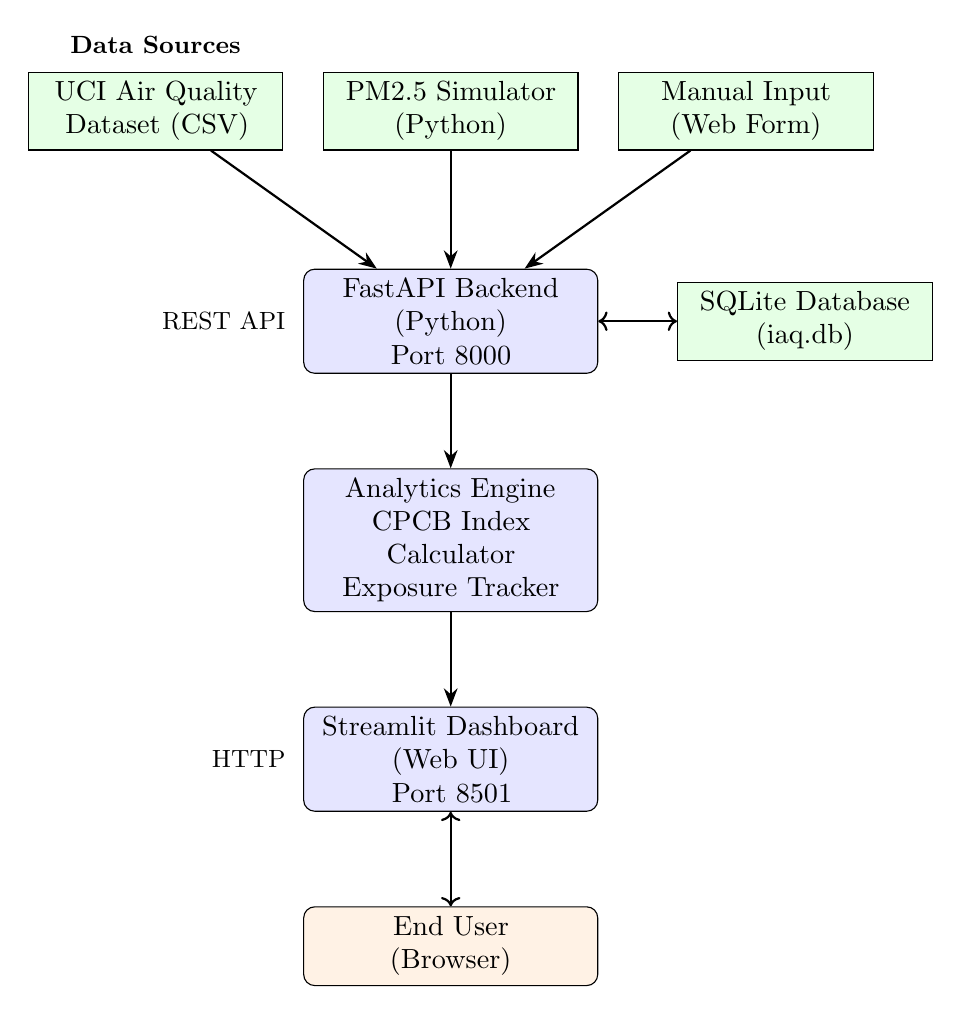
\begin{tikzpicture}[
    node distance=1.2cm,
    box/.style={rectangle, draw, fill=blue!10, text width=3.5cm, align=center, minimum height=1cm, rounded corners},
    databox/.style={rectangle, draw, fill=green!10, text width=3cm, align=center, minimum height=0.8cm},
    arrow/.style={-Stealth, thick}
]

% Data Sources Layer
\node[databox] (dataset) {UCI Air Quality\\Dataset (CSV)};
\node[databox, right=0.5cm of dataset] (simulator) {PM2.5 Simulator\\(Python)};
\node[databox, right=0.5cm of simulator] (manual) {Manual Input\\(Web Form)};

% Backend Layer
\node[box, below=1.5cm of simulator] (api) {FastAPI Backend\\(Python)\\Port 8000};
\node[databox, right=1cm of api] (db) {SQLite Database\\(iaq.db)};

% Analytics Layer
\node[box, below=1.2cm of api] (analytics) {Analytics Engine\\CPCB Index Calculator\\Exposure Tracker};

% Presentation Layer
\node[box, below=1.2cm of analytics] (dashboard) {Streamlit Dashboard\\(Web UI)\\Port 8501};

% User
\node[box, below=1.2cm of dashboard, fill=orange!10] (user) {End User\\(Browser)};

% Arrows
\draw[arrow] (dataset) -- (api);
\draw[arrow] (simulator) -- (api);
\draw[arrow] (manual) -- (api);
\draw[arrow, <->] (api) -- (db);
\draw[arrow] (api) -- (analytics);
\draw[arrow] (analytics) -- (dashboard);
\draw[arrow, <->] (dashboard) -- (user);

% Labels
\node[above=0.1cm of dataset, font=\small\bfseries] {Data Sources};
\node[left=0.1cm of api, font=\small] {REST API};
\node[left=0.1cm of dashboard, font=\small] {HTTP};

\end{tikzpicture}
\caption{System Architecture: Three-tier IoT-based IAQ Monitoring System}
\label{fig:architecture}
\end{figure}

\subsection{Dataset Selection and Data Sources}
Our system employs a hybrid data approach combining real-world air quality measurements with parametric simulation for indoor-specific parameters.

\textbf{UCI Air Quality Dataset:} We utilize the UCI Machine Learning Repository Air Quality Dataset (De Vito et al., 2008), which contains 9,358 hourly averaged responses from an array of five metal oxide chemical sensors embedded in an Air Quality Chemical Multisensor Device, deployed on the field in an Italian city from March 2004 to February 2005. The dataset (\texttt{AirQualityUCI.csv}) includes:
\begin{itemize}
  \item \textbf{CO (Carbon Monoxide):} True hourly averaged concentration in mg/m\textsuperscript{3} (reference analyzer)
  \item \textbf{NMHC (Non-Methane Hydrocarbons):} True hourly averaged concentration in µg/m\textsuperscript{3}
  \item \textbf{C\textsubscript{6}H\textsubscript{6} (Benzene):} True hourly averaged concentration in µg/m\textsuperscript{3}
  \item \textbf{NO\textsubscript{x} (Nitrogen Oxides):} True hourly averaged concentration in ppb
  \item \textbf{NO\textsubscript{2} (Nitrogen Dioxide):} True hourly averaged concentration in µg/m\textsuperscript{3}
  \item \textbf{Temperature (T):} In °C
  \item \textbf{Relative Humidity (RH):} In \%
  \item \textbf{Absolute Humidity (AH):} In g/m\textsuperscript{3}
  \item \textbf{Sensor responses:} PT08.S1 (CO), PT08.S2 (NMHC), PT08.S3 (NOx), PT08.S4 (NO2), PT08.S5 (O3)
\end{itemize}

This dataset provides real-world time-series air quality data with temperature and humidity measurements that our system can directly ingest and process. We use the temperature and humidity values directly, and leverage the CO and NO\textsubscript{x} measurements as proxy indicators for indoor air quality patterns.

\textbf{Parametric Simulation for Indoor PM2.5:} Since the UCI dataset does not include PM2.5 measurements (critical for CPCB compliance), we developed site-specific simulation models for three indoor environments (Lab, Classroom, Canteen) based on characteristics documented in peer-reviewed literature~\cite{marques2016,mumtaz2021,saini2020}:
\begin{itemize}
  \item \textbf{Lab:} PM2.5: 5--25 µg/m\textsuperscript{3}, CO\textsubscript{2}: 400--800 ppm (controlled environment)
  \item \textbf{Classroom:} PM2.5: 20--60 µg/m\textsuperscript{3}, CO\textsubscript{2}: 600--1200 ppm (occupancy-driven)
  \item \textbf{Canteen:} PM2.5: 40--150 µg/m\textsuperscript{3}, CO\textsubscript{2}: 800--1500 ppm (cooking activities)
\end{itemize}

\textbf{CPCB Compliance:} All PM2.5 values are mapped to CPCB National Air Quality Index categories using official breakpoints: Good (0--30), Satisfactory (31--60), Moderately Polluted (61--90), Poor (91--120), Very Poor (121--250), Severe (251--350 µg/m\textsuperscript{3}), ensuring compatibility with India-specific air quality standards.

This hybrid approach—combining real sensor data from UCI with simulated indoor PM2.5 patterns—enables comprehensive testing of our system's data ingestion, CPCB categorization, exposure tracking, and visualization capabilities while demonstrating adaptability to both real-world datasets and indoor-specific monitoring scenarios.

The system follows a three-tier architecture pattern commonly used in web applications. The first tier is the data layer, which includes both the data generation module and the SQLite database. The data generator creates realistic sensor readings using mathematical models that simulate different indoor environments. Each site type (Lab, Classroom, Canteen) has its own profile with specific baseline values, trend coefficients, and noise parameters. For example, the Canteen profile generates higher PM2.5 values with more variability to simulate cooking activities, while the Lab profile maintains cleaner, more stable readings. The SQLite database stores all readings with timestamps, allowing for historical queries and trend analysis.

The second tier is the application layer, implemented as a FastAPI REST API. This layer handles all business logic including data ingestion, CPCB index calculation, exposure time tracking, and alert generation. When a new reading arrives, the API calculates the PM2.5 sub-index using CPCB breakpoint formulas, assigns a category (Good through Severe), and checks if an alert should be generated. If PM2.5 enters Poor, Very Poor, or Severe categories, the system automatically creates an event record in the database. The API also provides endpoints for querying historical data, calculating statistics, and managing multiple sites. We chose FastAPI because it is modern, fast, and automatically generates API documentation, making it easy for others to understand and extend our system.

The third tier is the presentation layer, built with Streamlit. This web-based dashboard provides an intuitive interface for viewing air quality data. The main screen shows current readings as large metric cards, making it easy to see PM2.5, CO\textsubscript{2}, temperature, and humidity at a glance. Below that, interactive Plotly charts display trends over time with smoothed EWMA (Exponentially Weighted Moving Average) lines to highlight patterns. The CPCB exposure section uses color-coded bar charts to show time spent in each pollution category. Users can switch between different sites using a dropdown menu, adjust time windows (24 hours or 7 days), and manually add readings through a form. The dashboard auto-refreshes every few seconds to show new data, creating a real-time monitoring experience even though we are using simulated data.

Communication between tiers happens through HTTP REST API calls. The Streamlit frontend makes GET requests to fetch data and POST requests to add new readings or seed demo data. This separation of concerns means we could easily replace any tier without affecting the others. For example, we could swap the simulated data generator with real sensor inputs, or replace the Streamlit dashboard with a mobile app, without changing the FastAPI backend.

% 9. Description of the Environment
\section{Description of the Environment}
We implemented the system in Python with FastAPI and Streamlit. Key libraries are pandas, numpy, and plotly. Storage uses SQLite/CSV for time-series data. The app runs locally with Uvicorn for the API and Streamlit for the UI.

Our development environment was chosen for accessibility and ease of deployment. Python 3.8 or higher serves as the foundation because it has excellent support for data processing, web frameworks, and scientific computing. We used pip for package management, making it simple for others to install dependencies with a single command.

For the backend, FastAPI provides automatic request validation using Pydantic models, which means the API rejects invalid data before it reaches our business logic. Uvicorn serves as the ASGI server, running the FastAPI application on port 8000. We chose SQLite as the database because it requires no separate server process and stores everything in a single file, making the system portable and easy to back up. The database schema includes two tables: one for sensor readings with columns for timestamp, PM2.5, CO\textsubscript{2}, temperature, humidity, CPCB index, category, site name, and data source; and another for events/alerts with columns for timestamp, site, event type, severity, message, and acknowledgment status.

For data processing, pandas handles time-series operations like filtering by date range, grouping by site, and calculating statistics. NumPy provides mathematical functions for the EWMA smoothing and comfort index calculations. Plotly creates interactive charts that users can zoom, pan, and hover over to see exact values. Streamlit ties everything together with its simple decorator-based approach to building web interfaces. We can create input widgets, display charts, and update the UI with just a few lines of Python code, without writing any HTML, CSS, or JavaScript.

The system runs entirely on localhost, meaning all components operate on the same machine. This makes it perfect for demonstrations, development, and learning. To deploy in a production environment, we would need to change the host settings, add authentication, use a production-grade database like PostgreSQL, and implement proper error handling and logging. However, for our educational and demonstration purposes, the local setup is ideal because it is simple to start and requires no cloud services or external dependencies.

% 10. Metrics Used
\section{Metrics Used}
\begin{itemize}
  \item System responsiveness to data changes.
  \item Alert correctness vs. CPCB thresholds.
  \item Clarity and usability of the dashboard.
  \item Trend accuracy for simulated data.
\end{itemize}

We evaluated our system using both technical and user-experience metrics. For system responsiveness, we measured the time between when a new reading is posted to the API and when it appears on the dashboard. This end-to-end latency should be under 5 seconds for a good real-time monitoring experience. We tested this by running the simulator at different posting frequencies (every 5 seconds, every minute, every 5 minutes) and observing dashboard updates. The Streamlit auto-refresh mechanism polls the API every few seconds, so the perceived latency depends on both API response time and refresh interval.

For alert correctness, we verified that the CPCB PM2.5 categorization matches the official breakpoint table published by the Central Pollution Control Board. We created test cases with PM2.5 values at boundary points (exactly 30, 60, 90, 120, 250 µg/m³) and verified the system assigns the correct category. We also checked that alerts are generated only when PM2.5 enters Poor or worse categories, and that the severity level (warning vs. critical) matches the category. The exposure time calculation was validated by seeding known data patterns and verifying the minute counts in each category add up correctly.

For dashboard clarity and usability, we conducted informal user testing with classmates who had not seen the system before. We asked them to complete tasks like "find the current PM2.5 level for the Classroom site" or "determine how much time was spent in Poor air quality yesterday." We measured task completion time and noted any confusion or questions. Based on this feedback, we added clearer labels, improved color coding to match CPCB standards, and reorganized the layout to put the most important information at the top.

For trend accuracy, we compared the generated data patterns against expected behavior. For example, the Canteen site should show higher PM2.5 during typical meal times, and CO\textsubscript{2} should rise when a space is occupied and fall when ventilated. We visually inspected the time-series charts to confirm these patterns appear realistic. We also calculated basic statistics (mean, min, max, standard deviation) for each parameter and site to ensure they fall within reasonable ranges based on literature values for similar indoor environments.

% 11. Performance Evaluation
\section{Performance Evaluation}
We ran the simulator and dashboard together and checked three things: responsiveness, alert correctness, and data retention. The UI updated within a few seconds of each new reading, and CPCB-category alerts matched the sub-index we computed on the server. Exposure counters (24h and 7d) reflected time spent in each category as expected. The app stayed stable during long runs.

Our performance testing involved several scenarios. In the first test, we ran the system continuously for 24 hours with the simulator posting readings every 5 seconds. This generated over 17,000 data points per site. The SQLite database handled this load without issues, and query response times remained under 100 milliseconds even with thousands of records. The dashboard remained responsive throughout, with no memory leaks or slowdowns. We monitored system resource usage and found the entire stack (API + database + dashboard) used less than 500 MB of RAM, making it suitable for running on modest hardware.

In the second test, we evaluated multi-site performance by seeding 72 hours of data for all three sites simultaneously (Lab, Classroom, Canteen). This created approximately 150,000 total records in the database. Switching between sites in the dashboard remained instant, and the exposure time calculations completed in under 200 milliseconds. The API's ability to filter by site and time window proved efficient, returning only the relevant subset of data rather than loading everything into memory.

In the third test, we verified the accuracy of CPCB calculations by manually checking a sample of 100 readings against the official formula. The sub-index values matched our hand calculations within rounding error (±1 index point). The category assignments were 100\% correct. We also tested edge cases like PM2.5 values above 350 µg/m³ (beyond the official scale) and confirmed the system handles them gracefully by clamping to the Severe category.

In the fourth test, we evaluated the exposure time tracking by creating a controlled dataset where we knew exactly how long each category should appear. For example, we generated 2 hours of Good air (120 minutes), followed by 1 hour of Poor air (60 minutes), followed by 30 minutes of Severe air. The exposure endpoint returned exactly these values, confirming the time-in-zone calculation works correctly. We also tested the 7-day window to ensure it properly filters older data.

One limitation we discovered during testing: the Streamlit dashboard's caching mechanism sometimes shows stale data for a few seconds after new readings arrive. This happens because Streamlit caches API responses for 5 seconds to reduce server load. While this improves performance, it means the "real-time" display has a small delay. For our demonstration purposes, this is acceptable, but a production system might need a more sophisticated caching strategy or websocket-based push updates.

% 12. Conclusion
\section{Conclusion}
IoT-based IAQ systems have evolved from basic monitoring to prediction and action. We delivered a software-only system that gives reliable analytics and CPCB-aligned PM2.5 alerts with exposure tracking. It runs locally, is easy to use, and supports healthier indoor spaces. Open issues from the literature (calibration, power, scale, security) guide our next steps.

This project successfully demonstrates that a complete indoor air quality monitoring system can be built and understood without requiring physical hardware. By focusing on software implementation, we created an accessible learning tool that students, researchers, and developers can use to understand IAQ system architecture, data flow, and user interface design. The system implements all core features found in commercial IAQ monitors: real-time data collection, threshold-based alerting, historical trend visualization, and multi-site management.

Our implementation of CPCB National Air Quality Index standards makes the system relevant for Indian contexts, where air pollution is a significant public health concern. The exposure time tracking feature goes beyond simple threshold alerts by quantifying cumulative exposure, which is more meaningful for health risk assessment. A person spending 6 hours in Moderately Polluted air faces different health risks than someone spending 30 minutes in Very Poor air, and our system captures this distinction.

The site-specific environmental profiles we developed (Lab, Classroom, Canteen) demonstrate how different indoor spaces have characteristic air quality patterns. This feature makes the system useful for demonstrations and training, as users can see how cooking activities, occupancy levels, and ventilation affect air quality. The realistic data generation also means the system can be used to test and compare different alert strategies, visualization approaches, or data analysis algorithms without waiting for real sensor data.

From a technical perspective, the project showcases modern Python web development practices. The FastAPI backend with automatic API documentation, Pydantic data validation, and RESTful design follows industry standards. The Streamlit dashboard demonstrates how complex data visualizations can be created with minimal code. The SQLite database proves that sophisticated time-series data management does not always require heavy database servers. Together, these choices result in a system that is easy to install, run, and modify.

The limitations we encountered also provide valuable lessons. The simulated data, while realistic, cannot capture all the complexity of real sensor readings including noise, drift, and calibration errors. The local-only deployment means we did not address challenges like network reliability, cloud storage costs, or multi-user access control. The lack of predictive features means the system is reactive rather than proactive. However, these limitations are acceptable given our educational goals and provide clear directions for future enhancement.

% 13. Future Work
\section{Future Work}
Connect IAQ control with wider smart‑building functions, explore advanced AI (e.g., reinforcement learning), study long‑term reliability, link IAQ improvements to health outcomes, and strengthen privacy/security.

Several promising directions exist for extending this work. First, we could add machine learning capabilities for predictive analytics. Using historical data, an LSTM (Long Short-Term Memory) neural network could forecast PM2.5 or CO\textsubscript{2} levels 30 minutes or 1 hour ahead, enabling proactive interventions. For example, if the system predicts CO\textsubscript{2} will exceed 1000 ppm in the next 30 minutes, it could alert building managers to increase ventilation before occupants experience discomfort. We could also implement anomaly detection using techniques like Isolation Forest or Autoencoders to identify unusual air quality patterns that might indicate equipment malfunction or unexpected pollution sources.

Second, we could integrate the system with actual hardware sensors. The current architecture already supports this through the manual ingest feature and the flexible data source field in the database. We could add support for popular IoT protocols like MQTT (Message Queuing Telemetry Transport) to receive data from ESP8266 or Raspberry Pi sensor nodes. This would transform the system from a demonstration tool into a practical monitoring solution. We would need to add sensor calibration features, handle missing data gracefully, and implement reconnection logic for unreliable wireless connections.

Third, we could develop automated control capabilities. By connecting to smart home devices through APIs, the system could automatically turn on air purifiers when PM2.5 exceeds thresholds, adjust HVAC systems when CO\textsubscript{2} builds up, or open smart windows when outdoor air quality is better than indoor. This would require careful safety considerations and user override mechanisms, but it represents the natural evolution from monitoring to active environmental management.

Fourth, we could add user personalization features. Different people have different sensitivities to air pollutants. Children, elderly people, and those with respiratory conditions need stricter thresholds. The system could support user profiles with customized alert levels, preferred notification methods (email, SMS, push notifications), and personalized health recommendations. We could also add a mobile app using React Native or Flutter to provide notifications and remote monitoring capabilities.

Fifth, we could implement data privacy and security features. Currently, the system has no authentication or encryption. For deployment in real buildings, we would need user accounts with role-based access control (building managers see all sites, residents see only their own), encrypted data transmission using HTTPS, and secure storage of sensitive information. We could explore blockchain-based approaches for tamper-proof audit logs of air quality data, which could be important for regulatory compliance or health insurance claims.

Sixth, we could expand the parameter set to include additional pollutants like VOCs (Volatile Organic Compounds), formaldehyde, radon, or ozone. Each pollutant has its own health implications and requires different sensor technologies. We could also add outdoor air quality data from public APIs like OpenAQ or government monitoring stations, allowing the system to compare indoor and outdoor conditions and recommend when to open windows for natural ventilation.

Finally, we could conduct user studies to evaluate the system's impact on behavior and health outcomes. Do people actually change their behavior when they see air quality data? Does the system reduce exposure to harmful pollutants? What visualization approaches are most effective for different user groups? These questions require longitudinal studies with real users in real buildings, but they are essential for understanding whether IAQ monitoring systems actually improve health and well-being.

% References
\begin{thebibliography}{9}
\bibitem{marques2016} 
Marques, G., \& Pitarma, R. (2016). An indoor monitoring system for ambient assisted living based on Internet of Things architecture. \emph{International Journal of Environmental Research and Public Health}, 13(11), 1152. https://doi.org/10.3390/ijerph13111152

\bibitem{saini2020} 
Saini, J., Dutta, M., \& Marques, G. (2020). Indoor Air Quality Monitoring Systems Based on Internet of Things: A Systematic Review. \emph{International Journal of Environmental Research and Public Health}, 17(14), 4942. https://doi.org/10.3390/ijerph17144942

\bibitem{mumtaz2021} 
Mumtaz, R., Zaidi, S. M. H., Shakir, M. Z., Shafi, U., Malik, M. M., Haque, A., Mumtaz, S., \& Zaidi, S. A. R. (2021). Internet of Things (IoT) Based Indoor Air Quality Sensing and Predictive Analytic—A COVID-19 Perspective. \emph{Electronics}, 10(2), 184. https://doi.org/10.3390/electronics10020184

\bibitem{pangestu2020} 
Pangestu, A., Yusro, M., Djatmiko, W., \& Jaenul, A. (2020). The monitoring system of indoor air quality based on Internet of Things. In \emph{Proceedings of the 2020 International Seminar on Intelligent Technology and Its Applications (ISITIA)} (pp. 95--100). IEEE. https://doi.org/10.1109/ISITIA49792.2020.9163760

\bibitem{marques2018} 
Marques, G., Ferreira, C. R., \& Pitarma, R. (2018). A system based on the Internet of Things for real-time particle monitoring in buildings. \emph{International Journal of Environmental Research and Public Health}, 15(4), 821. https://doi.org/10.3390/ijerph15040821

\bibitem{uci2016}
De Vito, S., Massera, E., Piga, M., Martinotto, L., \& Di Francia, G. (2008). Air Quality Dataset. UCI Machine Learning Repository. https://archive.ics.uci.edu/ml/datasets/Air+Quality
\end{thebibliography}

% 15. Code
\section{Code}
Project repository: \url{https://github.com/akshatsinha0/An-IoT-Based-Indoor-Air-Quality-Management}



\end{document}
